%%%%%%%%%%%%%%%%%%%%%%%%%%%%%%%%%%%%%%%%%
% Short Sectioned Assignment
% LaTeX Template
% Version 1.0 (5/5/12)
%
% This template has been downloaded from:
% http://www.LaTeXTemplates.com
%
% Original author:
% Frits Wenneker (http://www.howtotex.com)
%
% License:
% CC BY-NC-SA 3.0 (http://creativecommons.org/licenses/by-nc-sa/3.0/)
%
%%%%%%%%%%%%%%%%%%%%%%%%%%%%%%%%%%%%%%%%%

%----------------------------------------------------------------------------------------
%	PACKAGES AND OTHER DOCUMENT CONFIGURATIONS
%----------------------------------------------------------------------------------------

\documentclass[paper=a4, fontsize=11pt]{scrartcl} % A4 paper and 11pt font size

\usepackage[T1]{fontenc} % Use 8-bit encoding that has 256 glyphs
%\usepackage{fourier} % Use the Adobe Utopia font for the document - comment this line to return to the LaTeX default
\usepackage[english]{babel} % English language/hyphenation
\usepackage{amsmath,amsfonts,amsthm} % Math packages
\usepackage{bm}
\usepackage{lipsum} % Used for inserting dummy 'Lorem ipsum' text into the template
\usepackage{graphicx} % This one is for pictures
\usepackage{sectsty} % Allows customizing section commands
\allsectionsfont{\centering \normalfont\scshape} % Make all sections centered, the default font and small caps
\usepackage{color}

\usepackage{fancyhdr} % Custom headers and footers
\pagestyle{fancyplain} % Makes all pages in the document conform to the custom headers and footers
\fancyhead{} % No page header - if you want one, create it in the same way as the footers below
\fancyfoot[L]{} % Empty left footer
\fancyfoot[C]{} % Empty center footer
\fancyfoot[R]{\thepage} % Page numbering for right footer
\renewcommand{\headrulewidth}{0pt} % Remove header underlines
\renewcommand{\footrulewidth}{0pt} % Remove footer underlines
\setlength{\headheight}{13.6pt} % Customize the height of the header

%\numberwithin{equation}{section} % Number equations within sections (i.e. 1.1, 1.2, 2.1, 2.2 instead of 1, 2, 3, 4)
%\numberwithin{figure}{section} % Number figures within sections (i.e. 1.1, 1.2, 2.1, 2.2 instead of 1, 2, 3, 4)
%\numberwithin{table}{section} % Number tables within sections (i.e. 1.1, 1.2, 2.1, 2.2 instead of 1, 2, 3, 4)

%\setlength\parindent{0pt} % Removes all indentation from paragraphs - comment this line for an assignment with lots of text

%----------------------------------------------------------------------------------------
%	TITLE SECTION
%----------------------------------------------------------------------------------------

\newcommand{\horrule}[1]{\rule{\linewidth}{#1}} % Create horizontal rule command with 1 argument of height

\title{	
\normalfont \normalsize 
\textsc{Columbia University -- Fall 2013} \\ [25pt] % Your university, school and/or department name(s)
\horrule{0.5pt} \\[0.4cm] % Thin top horizontal rule
\huge Machine Learning Homework \#2\\ % The assignment title
\horrule{2pt} \\[0.5cm] % Thick bottom horizontal rule
}

\author{Joe Ellis - jge2105} % Your name

\date{\normalsize\today} % Today's date or a custom date

\begin{document}

\maketitle % Print the title

%----------------------------------------------------------------------------------------
%	PROBLEM 1
%----------------------------------------------------------------------------------------

\section{Problem 1}



\section{Problem 2}

A stationary kernel is some kernel such that the kernel result is translation invariant, we denote this as $K(x,z) = K_s(x-z)$.  We have two examples of stationary kernels for this problem.  The first example is the exponential kernel, $K_e(x,z) = e^{(-\frac{||x-z||}{\theta})}$, and the second example is the gaussian kernel, which is $K_g(x,z) = e^{(-\frac{||x-z||^2}{\theta})}$.

We will show that they are mercer kernels based on the definition given in the lecture slides, that a mercer kernel is a kernel which is kernel that takes two inputs and outputs a scalar via denoted as,

\begin{align}
k(x_1,x_2) = <\phi(x_i),\phi(x_2)> = \left\{
	\begin{array}{ll}
		\phi(x_i)^t\phi(x_2) & \mbox{for } finite \phi \\
		\int_t \phi(x_i,t)\phi(x_2,t) & \mbox{otherwise} 
	\end{array}
\right.
\end{align} 

Both of these are mercer kernels, because they both output scalar values, for both conditions.
Let's assume that $\phi$ is finite, and then we know that on the top of the exponential function we have a magnitude which is scalar divided by a scalar parameter $\theta$ which yields some scalar output value.
We also, know that the integral of the kernel provided is bounded due to the nature of the gaussian and exponential kernel, and therefore $\int_t \phi(x_i,t)\phi(x_2,t)$, is also bounded.  Therefore, both are mercer kernels.

Now let's show that both of these are stationary kernels.  We will translate both of the elements by adding some arbitrary variable $k$, which is of the same dimensionality of the inputs $x_1$ and $x_2$.  Therefore, for any k we want to show that the kernels are stationary under sum and product.  First, assume we sum the kernels together,

\begin{align}
K_{sum}(x,z) &= K_e(x,z)+K_g(x,z) \\
&= e^{(-\frac{||x-z||}{\theta})} + e^{(-\frac{||x-z||^2}{\theta})}, \\
&= K_{se}(x-z) + K_{sg}(x-z). \\
\end{align}

Since both values that we receive in the summation depend only on the lag vectors, then we find that they are stationary under summation.

Now let's show that these are also stationary kernels under multiplication.  For multiplicaiton we have,

\begin{align}
K_{mult}(x,z) &= K_e(x,z)K_g(x,z) \\
&= e^{(-\frac{||x-z||}{\theta})}e^{(-\frac{||x-z||^2}{\theta})}, \\
&=  e^{(-\frac{||x-z||+||x-z||^2}{\theta})}\\
\end{align}

Since the exponent of the above multiplication of the kernels also only depends on the value $x-z$, we have shown that these are also stationary under multiplication.

For the second part of this problem, we will explicitly find the $\phi$ function such that $K(x_1,x_2) = \phi(x_1)^t\phi(x_2) =  e^{(-|||x_1-x_2||^2}$.

\begin{align}
K(x_1,x_2) &= \phi(x_1)^t\phi(x_2) \\
&= e^{-||x_1-x_2||^2} \\
&= e^{-(x_1-x_2)(x_1-x_2)}\\
&= e^{-(x_1^{2} + x_2^{2} + 2x_1x_2)}
\end{align}



\section{Problem 3}

For this problem we calculated the gram matrix for a given kernel $f(x,\lambda,k)$.
We define $f(x,\lambda,k)$ as $0$ for $x < 0$, and $f(x,k,\lambda)=(\frac{k}{\lambda})(\frac{x}{\lambda})^{k-1}(e^{-(\frac{x}{\lambda})^k})$.
We define our kernel function $K(x_i,x_j) = F(x_i^tx_j,\lambda=0.75,k=3)$, where $F(x,\lambda,k) =\int^x_0 f(x,\lambda,k)\,dx$. 

When we integrate $(f(x,\lambda,k)$, we get for the indefinite integral, 

\begin{align}
\int f(x,\lambda,k) \,dx = F(x,\lambda,k) = -e^{(\frac{x}{l})^k}.
\end{align}

Therefore, using this knowledge and computing the definite integral between two points, we created a Matlab script to calculate the desired gram matrix.
The gram matrix can be seen here, 

\[ \left( \begin{array}{ccccc}
0.0698 & 0.0456 & 0.0104 & 0.0072 & 0.0635 \\
0.0456 & 0.0420 & 0.0043 & 0.0061 & 0.0191 \\
0.0104 & 0.0043 & 0.0053 & 0.0007 & 0.0080 \\
0.0072 & 0.0061 & 0.0007 & 0.0009 & 0.0039 \\
0.0635 & 0.0191 & 0.0080 & 0.0039 & 0.2478\end{array} \right)\] 

This is the gram matrix for the points given in problem 3.

\section{Problem 4}

Here we create an object recognition system using SVM for classification.
Multiple different SVM kernels were chosen and evaluated, and all of the kernels chosen were able to perform well with the proper parameters.  
We performed cross-validation across the data-set using a 50-50 train and test split for the sample data points.
We performed cross-validation with 10 random splits for each parameter to show the performance of the SVM with each different kernel.
Given the proper parameters we were able to get 100\% accuracy using each of the described kernels, and this is because the data provided to us was seperable.  
Figure ~\ref{fig:plot_2d} shows the positive and negative samples from our dataset plotted with respect to their first two dimensions.
We can see that they are seperable through a linear svm.

\begin{figure}
\centering
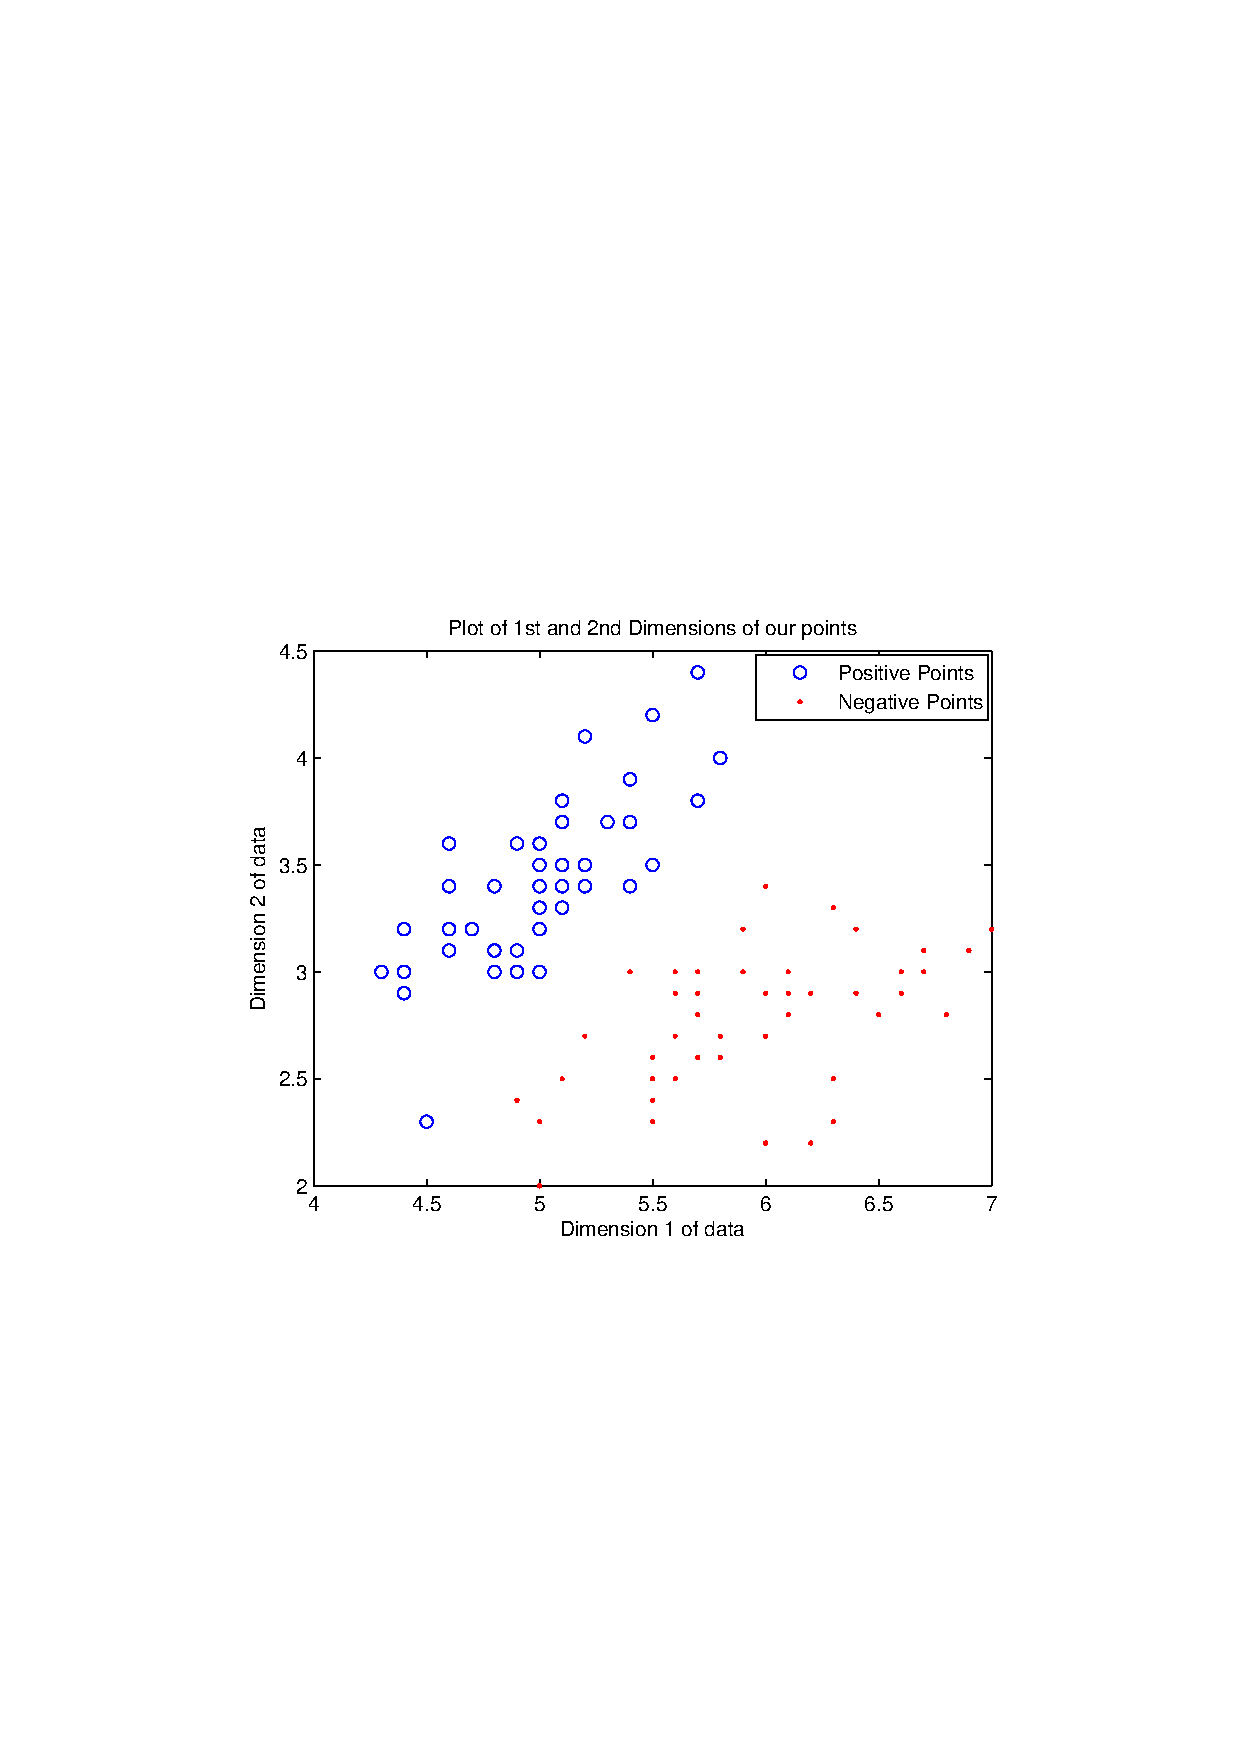
\includegraphics[scale=0.4]{serperability.jpg}
\caption{Plot of the 1st and 2nd dimensions of the dataset}
\label{fig:plot_2d}
\end{figure}

For classification we used linear, RBF, and polynomial SVM with different values for the cost variable (C), and the number of degrees for the polynomial function and the size of sigma in the RBF.
Each of these paramters effected the classification accruacy, but proper parameters for each kernel scheme could be found.
The results of a different parameters can be seen in the upcoming figures.

\begin{figure}
\centering
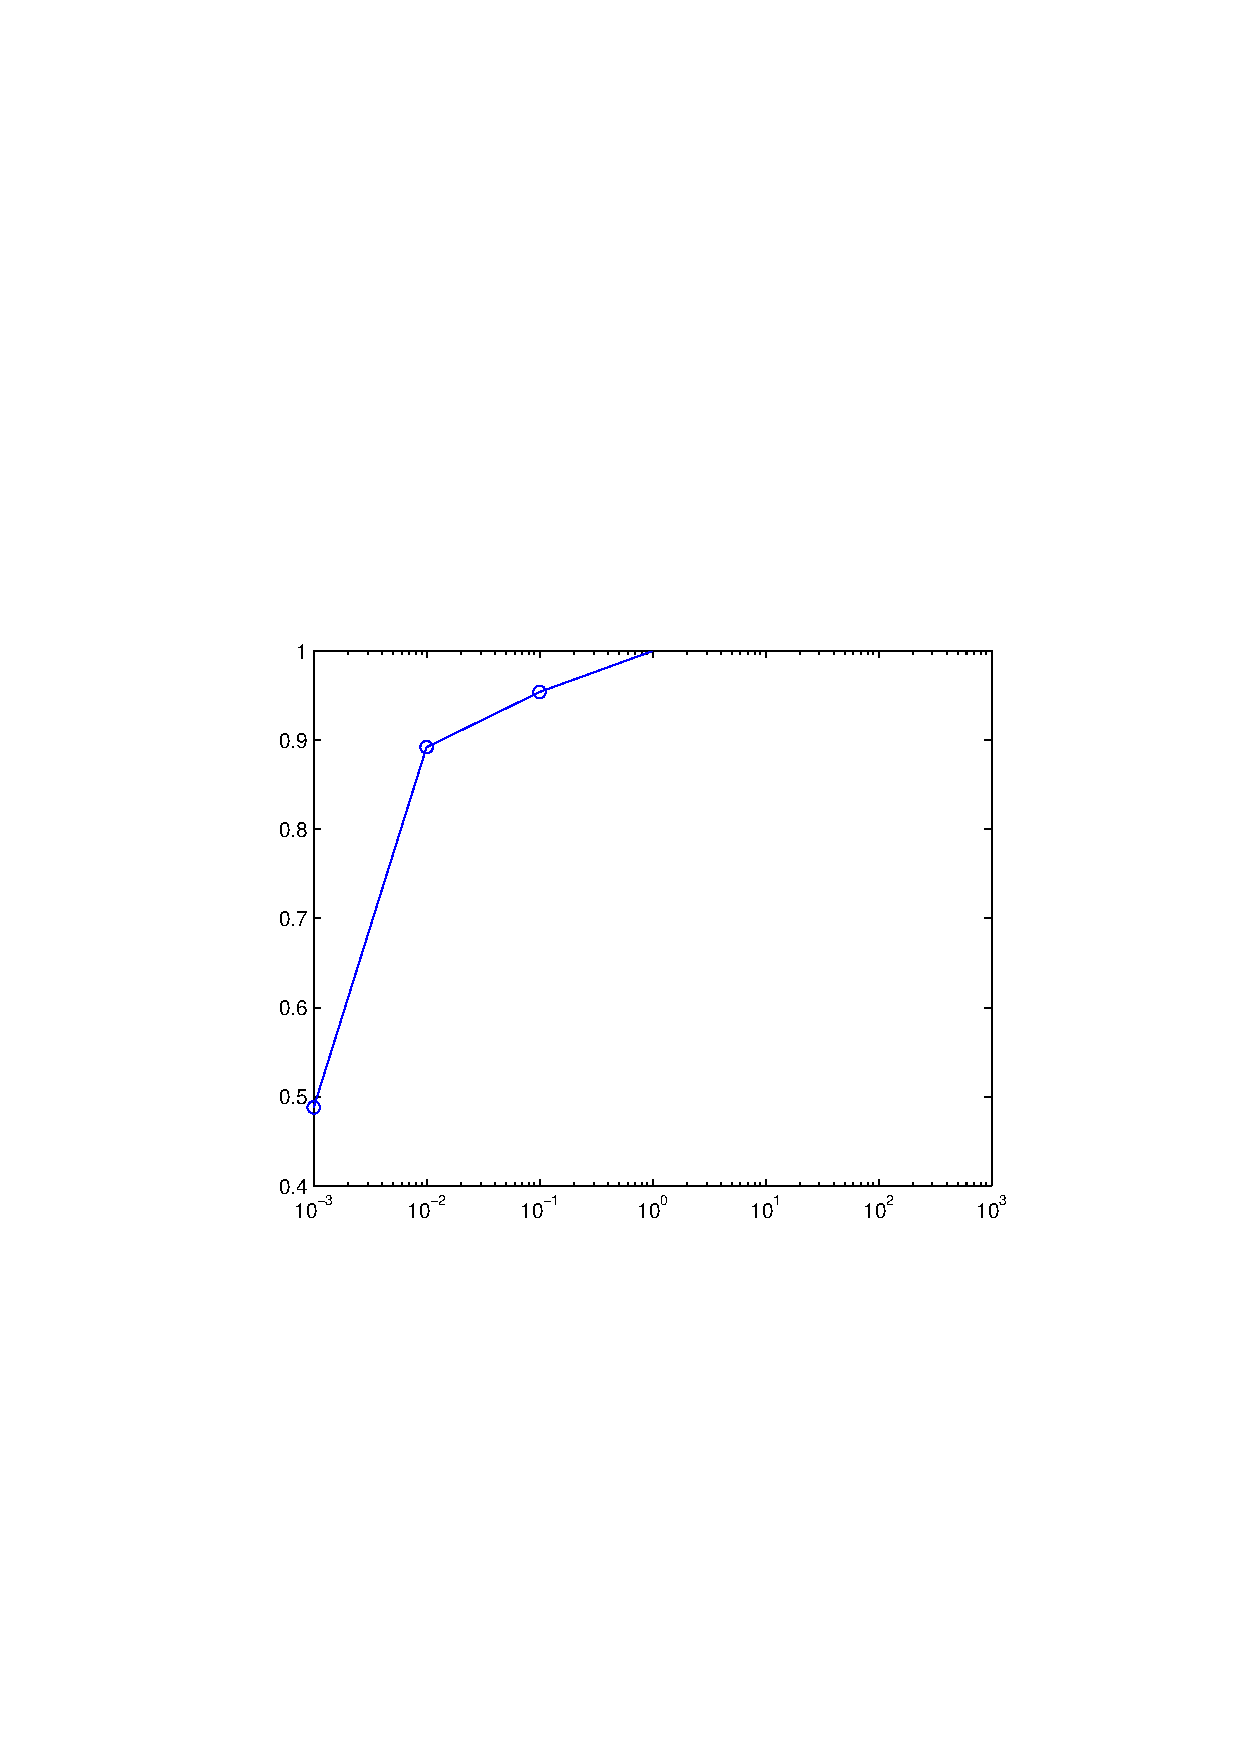
\includegraphics[scale=0.4]{linear.jpg}
\caption{Linear SVM classification accuracy for different parameters}
\label{fig:plot_2d}
\end{figure}

\begin{figure}
\centering
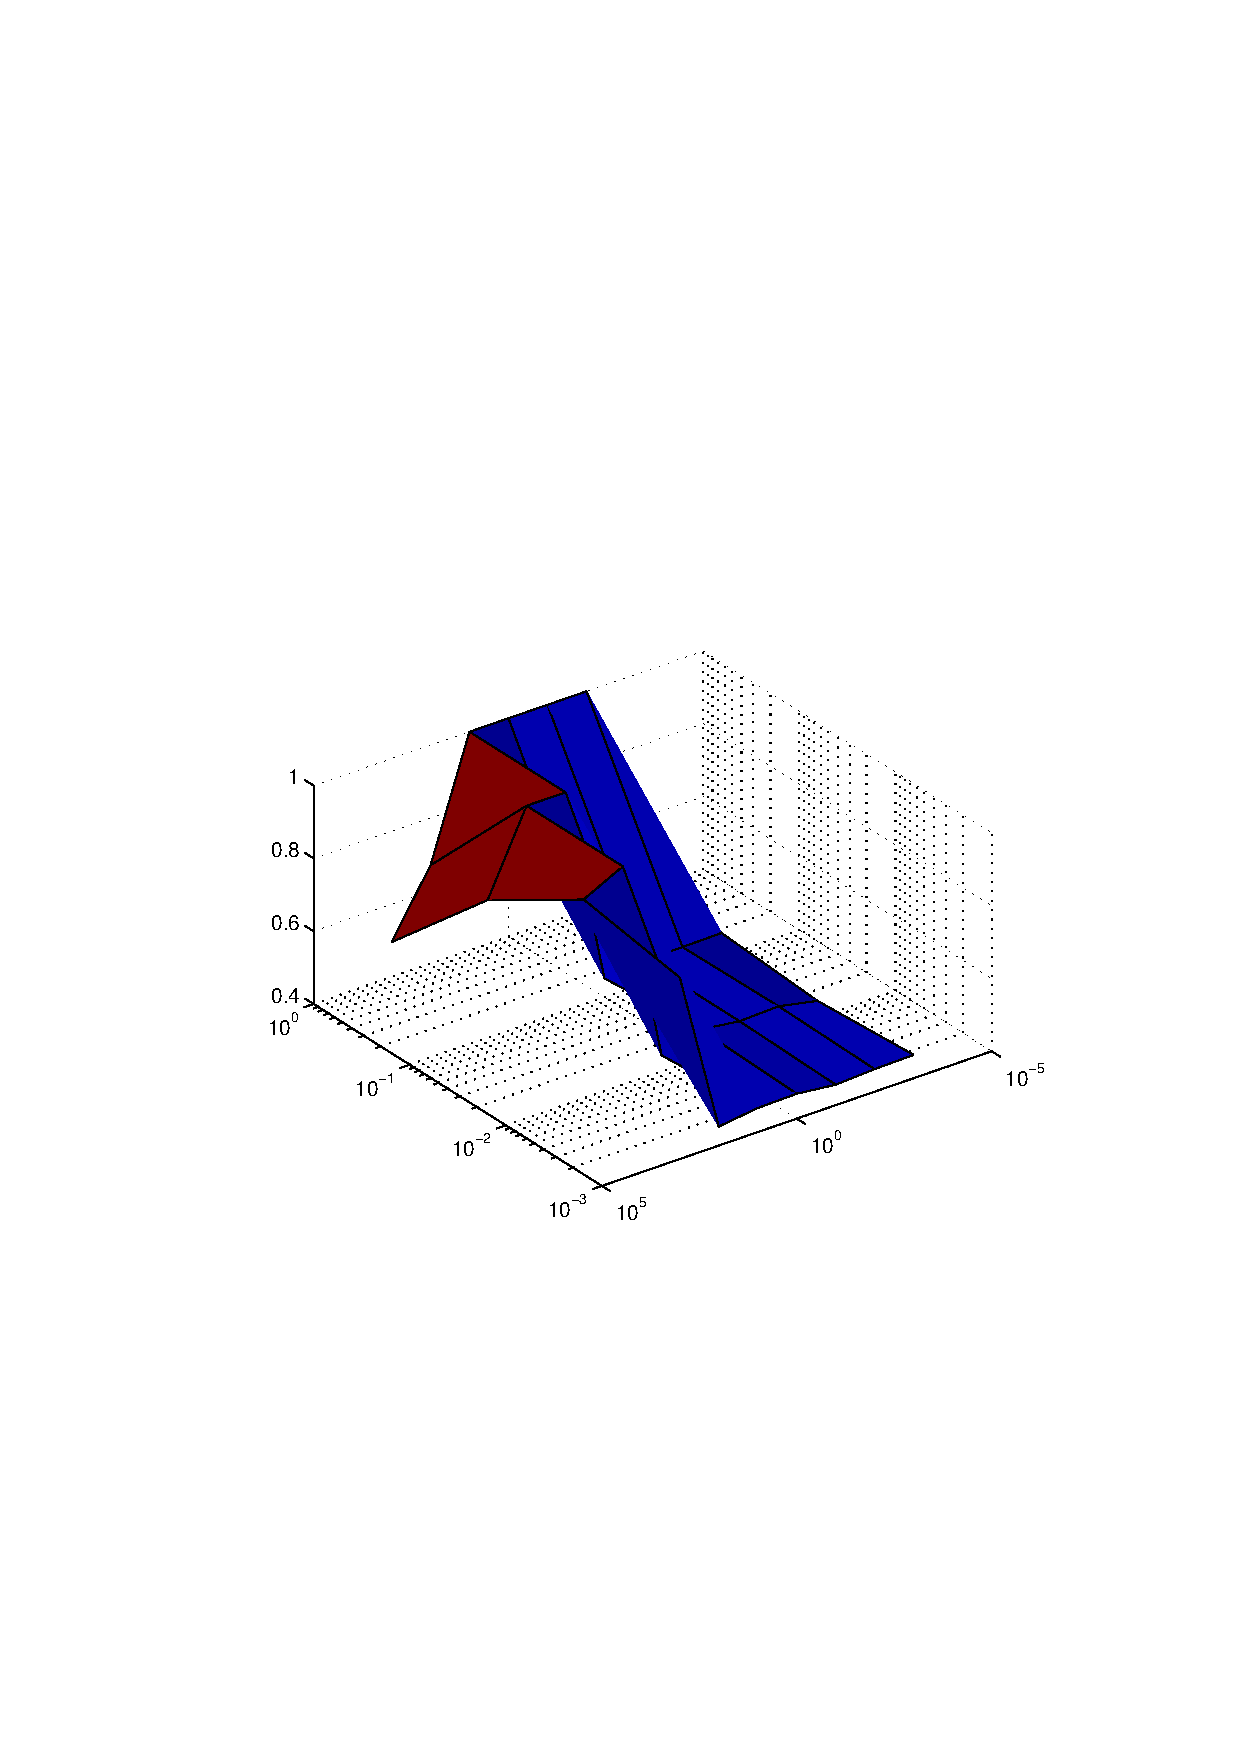
\includegraphics[scale=0.4]{RBF2.jpg}
\caption{RBF SVM classification accuracy for different parameters}
\label{fig:plot_2d}
\end{figure}

\begin{figure}
\centering
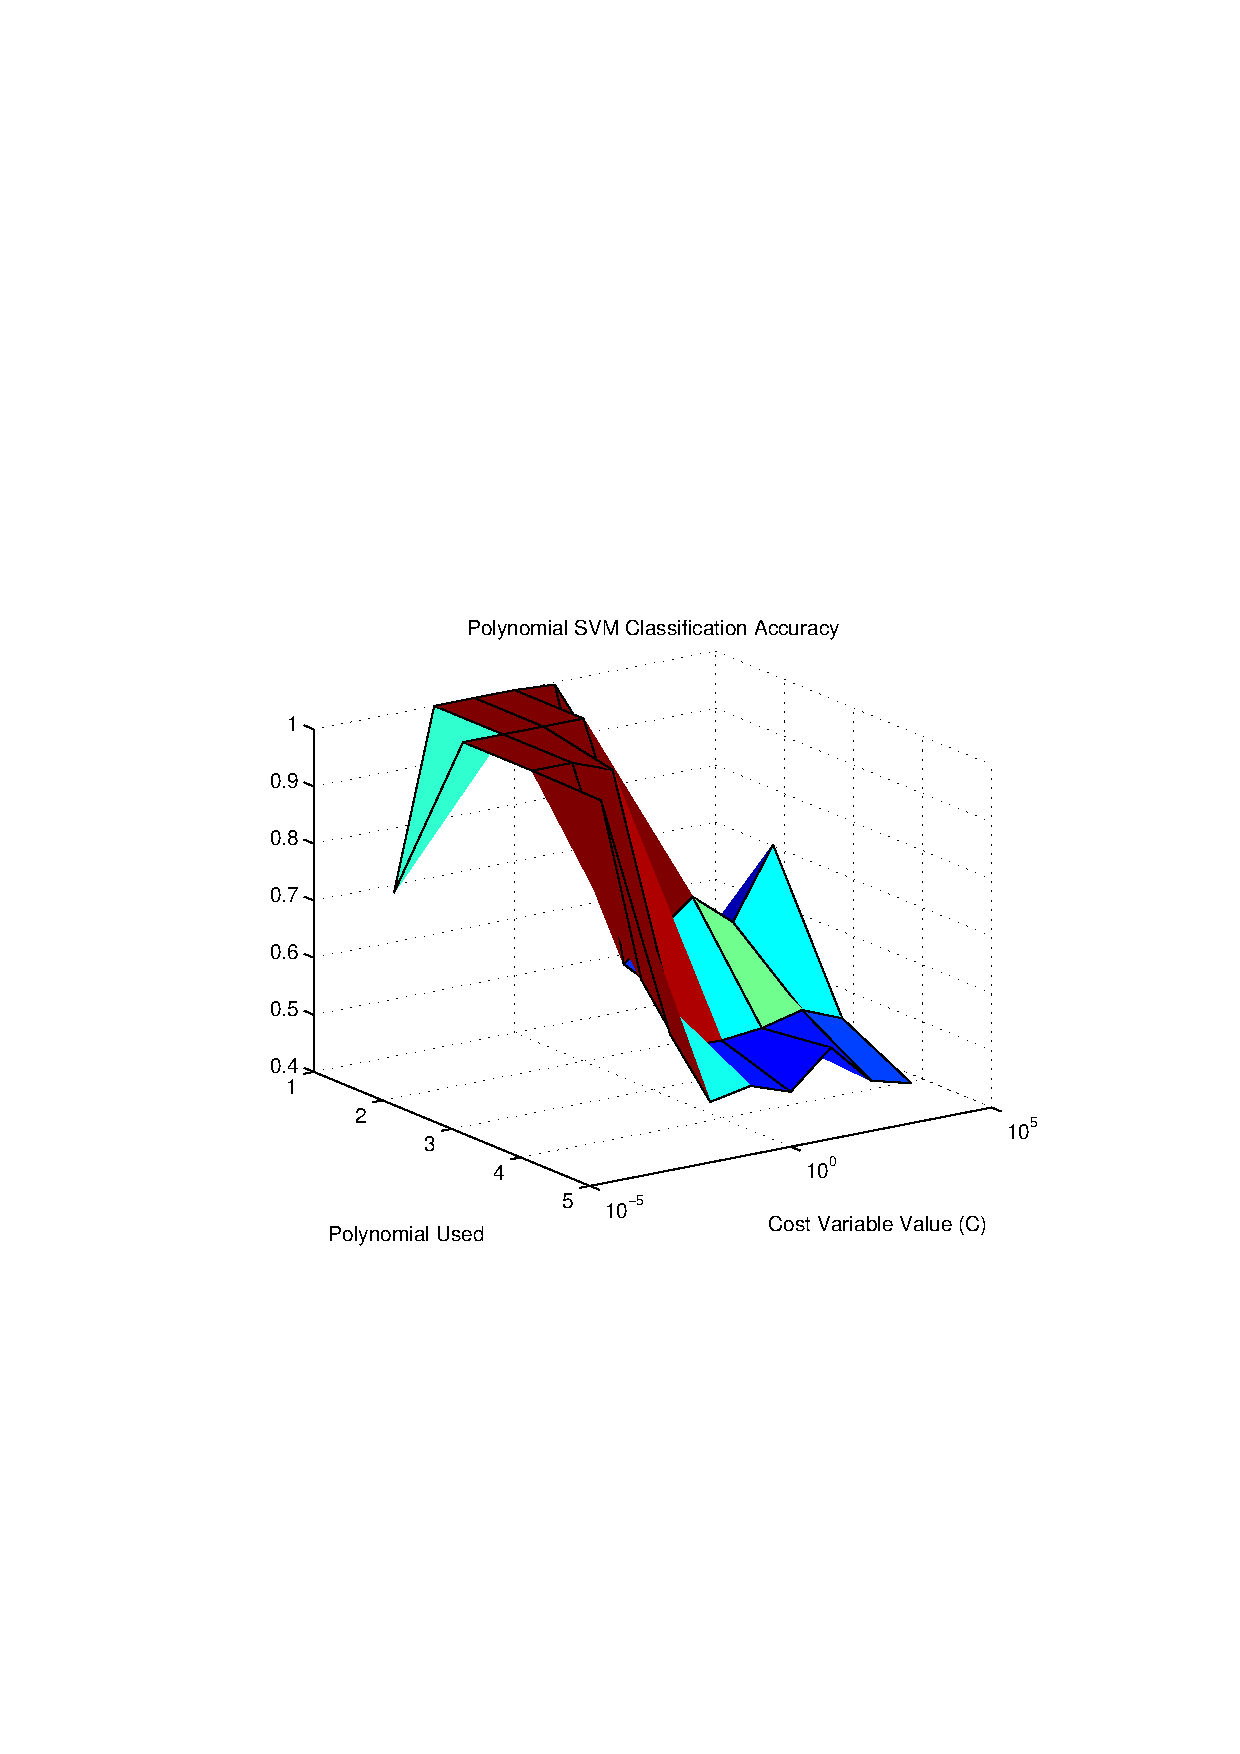
\includegraphics[scale=0.4]{Ploy.jpg}
\caption{Polynomial SVM classification accuracy for different parameters }
\label{fig:plot_2d}
\end{figure}

As you can see, we have found parameters for each type of kernel that achieves maximum accuracy. 
However, the kernel that in general used the least amount of support vectors, and was quickest in classification was the linear SVM.
Therefore, for this particular classification task I would reccomend using the linear SVM with $C=10$.
However, if the dataset is more difficult and not linearly seperable we would instead need to focus on using a more flexible kernel function such as the RBF.


\end{document}